\subsection{Models of the Atom}

The discovery of something so much smaller than the lightest atom threw Dalton's atomic theory out the window.
His theory claimed that everything in the universe was made up of atoms which would vary in size and mass based on the element .
These atoms could not be created or destroyed, but could rearrange themselves through chemical reactions.
It could be argued that Dalton's model was a progenitor for the idea of conservation of mass and energy\cite{Dalton}.
Despite being such an important idea, even before the discovery of electrons, the theory wasn't foolproof; it could not account for isotopes of the same element having different masses. 
The electron blew the idea wide apart.

A new theory that looked at the atom not as the smallest thing that could exist, but rather something that had other things inside in some sort of structure had to be developed.

The first problem to grapple with was that electrons are negatively charged while the atoms themselves are electrically neutral.
There were numerous models that tried to tackle this problem and one of the first was proposed by Thomson in 1904 as the plum pudding model.

To address this issue, the plum pudding model suggests that the electrons were suspended in a morass of positively charged particles
\footnote{Kind of like plums suspended in a pudding, hence the name of the model}
with the charge between the positive and negative equalling out to 0.
Thomson believed that the mass was evenly distributed throughout the atom\cite{Thomson_1907}.

\begin{figure}[H]
  % https://en.m.wikipedia.org/wiki/File:Plum_pudding_atom.svg
  \centering
  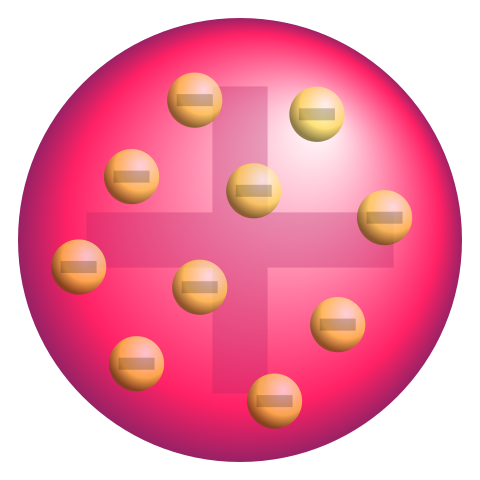
\includegraphics[width=100mm]{figures/plumPudding.png}
  \caption{Cartoon of plum pudding model\cite{PPmodel}}
  \label{plumPudding}
\end{figure}

The plum pudding model struggled to explain how these charged particles were so copacetic with each other despite being such small physical distances apart.
It was well known by then that opposite charges attract while alike charges repel \cite{Nagaoka}.
It also failed to provide any explanation of the spectral lines observed in hydrogen\cite{Thomson_1907}.
Darker clouds were still on the horizon for Thomson's plum pudding model.

Between 1906 and 1913, a number of alpha ($\alpha$) particle scattering experiments were performed by Hans Geiger and Ernest Marsden under the supervision of Ernest Rutherford, Langworthy Professor of Physics at the Victoria University of Manchester. 
These are known to us today as the Rutherford scattering experiments.
They designed experiments that involved firing a beam of $\alpha$ particles at metal foils of different thicknesses and materials to observe how the particles scattered in relation to the changes, although they ended up favoring gold foil for the experiments \cite{Tibbetts}. 
Based on the plum pudding model, it was expected that the $\alpha$ particles would not be deflected however, this turned out not to be the case at all.
To be fair, most of the $\alpha$ particles did indeed go straight through the gold foil, their trajectory not disturbed in the slightest.
A smaller fraction did get deflected, some by a small angle and others by a large one\cite{Belyaev_Ross}.
But the astonishing part was that an even smaller fraction, about 1 in 20000, shot right back at the direction the particle gun was shooting from\cite{Atomic_Nucleus}.

\begin{figure}[H]
  % https://en.wikipedia.org/wiki/Rutherford_scattering_experiments#/media/File:Geiger-Marsden_experiment_expectation_and_result.svg
  \centering
  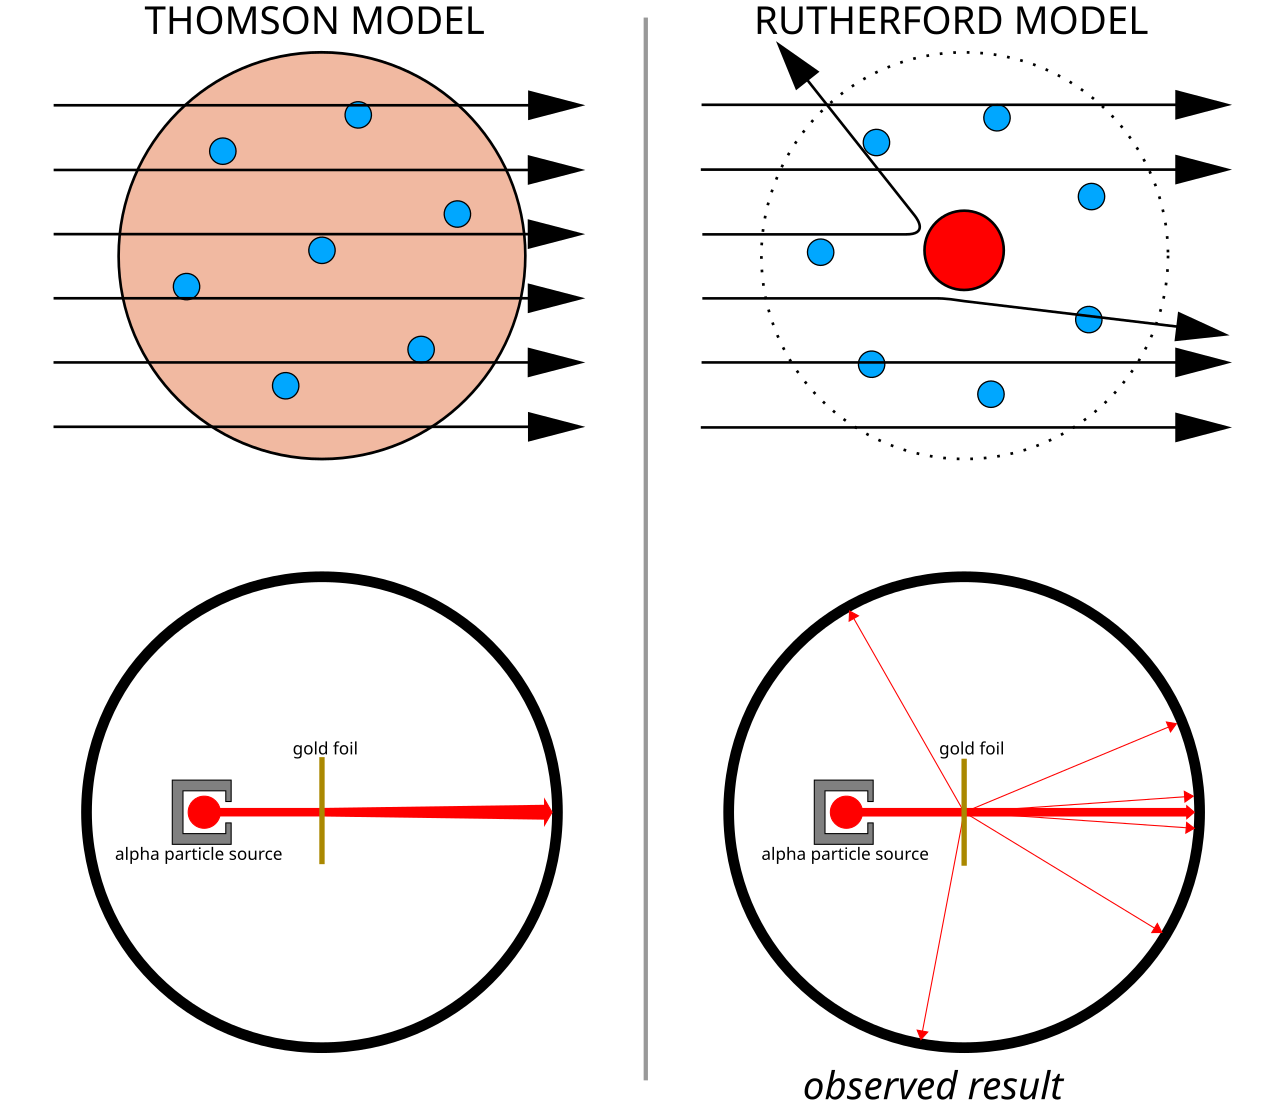
\includegraphics[width=100mm]{figures/goldFoil.png}
  \caption{Cartoon of Gold foil experiment\cite{GM_Experiment}}
  \label{goldFoil}
\end{figure}

So a new model was required to explain the discrepancies away.
Rutherford looked at the gold foil experiments and developed a new theory on the substructure of the atom\cite{Baily}.
He proposed in 1911 that atoms were mostly just empty space with a highly concentrated segment of mass at the center of the atom -- he called this central mass the nucleus of the atom.
In Rutherford's atomic model, the electrons orbit around the positively charged nucleus\cite{Rutherford_1911}.

\begin{figure}[H]
  % https://en.wikipedia.org/wiki/Rutherford_model#/media/File:Rutherford_atomic_planetary_model.svg
  \centering
  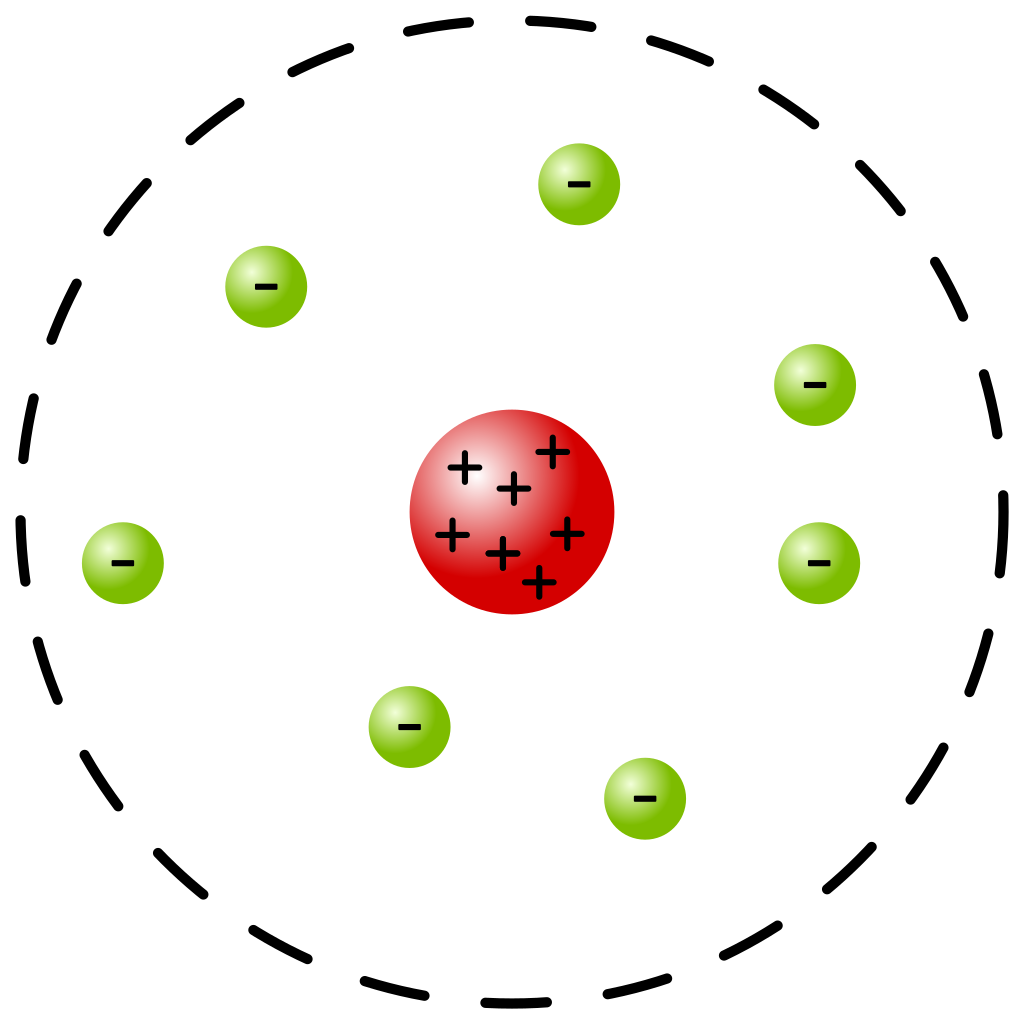
\includegraphics[width=100mm]{figures/rutherford.png}
  \caption{Rutherford's atomic model\cite{Rutherford_model}}
  \label{rutherford}
\end{figure}

Only, two little problems.
When things move in a circular orbit, they are accelerating. 
And if a charged particle is moving in an orbit like that, it should be constantly radiating energy.
This would lead the particle to eventually falling into the nucleus, making this model of the atom unstable.
It should also be emitting a continuous energy spectrum from the electrons, but hydrogen has discrete spectral lines\cite{Kopot}.

Bohr tried to come at this from an angle that resolved the spectral line issue with Rutherford's model.
Bohr proposed that electrons move in fixed orbits, thus explaining the discrete lines of the hydrogen spectra and that atoms emit light when an electron jumps from a higher energy level to a lower one \cite{Bohr_1913}.

\begin{figure}[H]
  % https://en.wikipedia.org/wiki/Bohr_model#/media/File:Bohr_atom_model.svg 
  \centering
  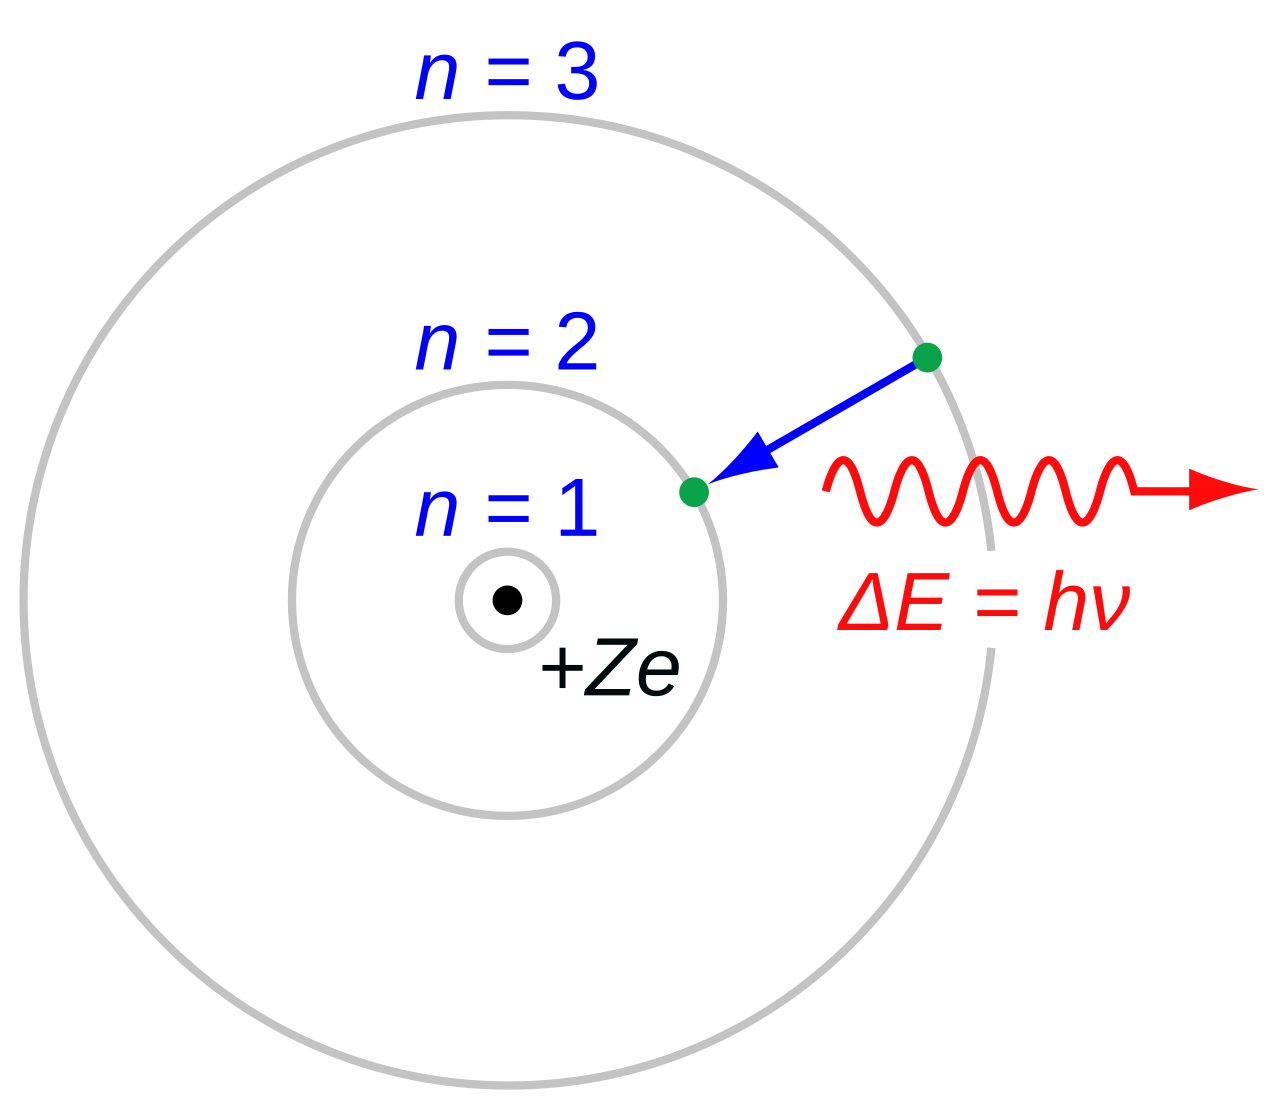
\includegraphics[width=100mm]{figures/bohr.png}
  \caption{Bohr's model of the hydrogen atom\cite{Bohr_model}}
  \label{bohr}
\end{figure}

This still doesn't explain away why the electron doesn't collapse into the nucleus.
However, it does a very good job of modelling hydrogen and hydrogen-like atoms under most normal conditions.
The other issue with Bohr's model is that it fails to address De-Broglie’s Hypothesis of the dual nature of matter.
To get there, we have to delve into the wonderful world of quantum mechanics.
